\section{Ejercicio 2}

% Defino un comando para trabajar mas comodo con subindices
\newcommand{\subindex}[1]{_{\ \ \color{red} #1}}

% El desarrollo de la primera expresión de 5 variables
% usando mintérminos se realiza en esta subsección
\subsection{Expresi\'on en mint\'erminos}
La subsecci\'on presente tratar\'a la siguiente expresi\'on caracterizada como:
\begin{equation*}
    f(e,d,c,b,a) = \sum m(0,2,4,7,8,10,12,16,18,20,23,24,25,26,27,28)
\end{equation*}


\subsubsection{Simplificación con Álgebra booleana}
En el siguiente desarrollo primero se escribe de forma completa la suma de productos que se describe en la expresi\'on
consignada, donde cada producto se compone de la combinaci\'on de entradas en cada estado indicado, de forma tal que el resultado 
de tal producto sea un estado l\'ogico activo, esto es, un '1' binario. Con el objetivo de proveer la mayor claridad posible en el desarrollo,
se subindican los t\'erminos, en donde el sub\'indice describe la identificaci\'on de un t\'ermino.

\begin{align*}
f(e,d,c,b,a) & =  \subindex{0} {\overline{e} \cdot \overline{d} \cdot \overline{c} \cdot \overline{b} \cdot \overline{a}}
+ \subindex{1} {\overline{e} \cdot \overline{d} \cdot \overline{c} \cdot b \cdot \overline{a}} 
+ \subindex{2} {\overline{e} \cdot \overline{d}  \cdot c \cdot \overline{b} \cdot \overline{a}}  
+ \subindex{3} {\overline{e} \cdot d \cdot \overline{c} \cdot \overline{b} \cdot \overline{a}} 
+ \subindex{4} {\overline{e} \cdot \overline{d} \cdot c \cdot b \cdot a} \\
& + \subindex{5} {\overline{e} \cdot d \cdot \overline{c} \cdot b \cdot \overline{a}} 
+ \subindex{6} {\overline{e} \cdot d \cdot c \cdot \overline{b} \cdot \overline{a}}
+ \subindex{7} {e \cdot \overline{d} \cdot \overline{c} \cdot \overline{b} \cdot \overline{a}} 
+ \subindex{8} {e \cdot \overline{d} \cdot \overline{c} \cdot b \cdot \overline{a}}
+ \subindex{9} {e \cdot \overline{d} \cdot c \cdot \overline{b} \cdot \overline{a}} \\
& + \subindex{10} {e \cdot \overline{d} \cdot c \cdot b \cdot a}
+ \subindex{11} {e \cdot d \cdot \overline{c} \cdot \overline{b} \cdot \overline{a}}
+ \subindex{12} {e \cdot d \cdot \overline{c} \cdot \overline{b} \cdot a} 
+ {\subindex{13} e \cdot d \cdot \overline{c} \cdot b \cdot \overline{a}} 
+ \subindex{14} {e \cdot d \cdot \overline{c} \cdot b \cdot a} \\
& + \subindex{15} {e \cdot d \cdot c \cdot \overline{b} \cdot \overline{a}}
\end{align*}

Luego se toman los t\'erminos de una manera adecuada de forma tal que se aplica sobre ellos la propiedad de abosrci\'on 
y luego se reducen, obteniendo como resultado la siguiente expresi\'on en la cual se subindican a izquierda y en rojo de d\'onde
fueron simplificados aplicando la absorci\'on.

\begin{align*}
f(e,d,c,b,a) & = \subindex{13,14} {e \cdot d \cdot \overline{c} \cdot b} 
+ \subindex{13,5}  {d \cdot \overline{c} \cdot b \cdot \overline{a}}
+ \subindex{13,8}  {e \cdot \overline{c} \cdot b \cdot \overline{a}}
+ \subindex{0,1}  {\overline{e} \cdot \overline{c} \cdot \overline{d} \cdot \overline{a}}
+ \subindex{0,2}  {\overline{e} \cdot \overline{d} \cdot \overline{b} \cdot \overline{a}}
+ \subindex{0,3}  {\overline{e} \cdot \overline{c} \cdot \overline{b} \cdot \overline{a}} \\
& + \subindex{3,6}  {\overline{e} \cdot d \cdot \overline{b} \cdot \overline{a}} 
+ \subindex{0,7}  {\overline{d} \cdot \overline{c} \cdot \overline{b} \cdot \overline{a}}
+ \subindex{2,9}  {\overline{d} \cdot c \cdot \overline{b} \cdot \overline{a}}
+ \subindex{3,11}  {d \cdot \overline{c} \cdot \overline{b} \cdot \overline{a}} 
+ \subindex{11,12}  {e \cdot d \cdot \overline{c} \cdot \overline{b}}
+ \subindex{11,15}  {e \cdot d \cdot \overline{b} \cdot \overline{a}} \\
& + \subindex{1,5}  {\overline{e} \cdot \overline{c} \cdot b \cdot \overline{a}}
+ \subindex{2,6}  {\overline{e} \cdot c \cdot \overline{b} \cdot \overline{a}} 
+ \subindex{3,5}  {\overline{e} \cdot d \cdot \overline{c} \cdot \overline{a}}
+ \subindex{7,8}  {e \cdot \overline{d} \cdot \overline{c} \cdot \overline{a}} 
+ \subindex{7,9}  {e \cdot \overline{d} \cdot \overline{b} \cdot \overline{a}}
+ \subindex{4,10}  {\overline{d} \cdot c \cdot b \cdot a}
\end{align*}

Con el fin de no recargar la notaci\'on y mantener el m\'etodo empleado para vincular aquellos
t\'erminos que son simplificados, se copian nuevamente la expresi\'on previa con una numeraci\'on nueva
que en este caso los identifica para su posterior simplificaci\'on.

\begin{align*}
f(e,d,c,b,a) & = \subindex{0} {e \cdot d \cdot \overline{c} \cdot b} 
+ \subindex{1}  {d \cdot \overline{c} \cdot b \cdot \overline{a}}
+ \subindex{2}  {e \cdot \overline{c} \cdot b \cdot \overline{a}}
+ \subindex{3}  {\overline{e} \cdot \overline{c} \cdot \overline{d} \cdot \overline{a}}
+ \subindex{4}  {\overline{e} \cdot \overline{d} \cdot \overline{b} \cdot \overline{a}}
+ \subindex{5}  {\overline{e} \cdot \overline{c} \cdot \overline{b} \cdot \overline{a}} \\
& + \subindex{6}  {\overline{e} \cdot d \cdot \overline{b} \cdot \overline{a}} 
+ \subindex{7}  {\overline{d} \cdot \overline{c} \cdot \overline{b} \cdot \overline{a}}
+ \subindex{8}  {\overline{d} \cdot c \cdot \overline{b} \cdot \overline{a}}
+ \subindex{9}  {d \cdot \overline{c} \cdot \overline{b} \cdot \overline{a}} 
+ \subindex{10}  {e \cdot d \cdot \overline{c} \cdot \overline{b}}
+ \subindex{11}  {e \cdot d \cdot \overline{b} \cdot \overline{a}} \\
& + \subindex{12}  {\overline{e} \cdot \overline{c} \cdot b \cdot \overline{a}}
+ \subindex{13}  {\overline{e} \cdot c \cdot \overline{b} \cdot \overline{a}} 
+ \subindex{14}  {\overline{e} \cdot d \cdot \overline{c} \cdot \overline{a}}
+ \subindex{15}  {e \cdot \overline{d} \cdot \overline{c} \cdot \overline{a}} 
+ \subindex{16}  {e \cdot \overline{d} \cdot \overline{b} \cdot \overline{a}}
+ \subindex{17}  {\overline{d} \cdot c \cdot b \cdot a}
\end{align*}

Repitiendo la modalidad, se simplifican algunos de los t\'erminos aplicando la regla de la absorci\'on,
se indican en los t\'erminos resultantes aquellos que fueron juntados.

\begin{align*}
f(e,d,c,b,a) & = \subindex{0,10} {e \cdot d \cdot \overline{c}}
+ \subindex{1,9} {\color{blue} d \cdot \overline{c} \cdot \overline{a}}
+ \subindex{8,9} {\overline{d} \cdot \overline{b} \cdot \overline{a}}
+ \subindex{4,6} {\color{brown} \overline{e} \cdot \overline{b} \cdot \overline{a}}
+ \subindex{2,12} {\overline{c} \cdot b \cdot \overline{a}}
+ \subindex{3,14} {\overline{e} \cdot \overline{c} \cdot \overline{a}}
+ \subindex{5,13} {\overline{e} \cdot \overline{b} \cdot \overline{a}} \\
& + \subindex{11,16} {\color{brown} e \cdot \overline{b} \cdot \overline{a}}
+ \subindex{17} {\overline{d} \cdot c \cdot b \cdot a}
+ \subindex{3,15} {\color{blue} \overline{d} \cdot \overline{c} \cdot \overline{a}}
\end{align*}

En la \'ultima expresi\'on hay dos pares de t\'erminos de colores azul y marr\'on, sobre los cuales
puede aplicarse propiedad de la absorci\'on nuevamente y se reescribe adecuadamente como sigue:

\begin{align*}
f(e,d,c,b,a) & = {e \cdot d \cdot \overline{c}}
+ {\color{blue} \overline{b} \cdot \overline{a}}
+ {\color{brown} \overline{c} \cdot \overline{a}}
+ {\color{blue} \overline{d} \cdot \overline{b} \cdot \overline{a}}
+ {\color{brown} \overline{c} \cdot b \cdot \overline{a}}
+ {\color{brown} \overline{e} \cdot \overline{c} \cdot \overline{a}}
+ {\color{blue} \overline{e} \cdot \overline{b} \cdot \overline{a}}
+ {\overline{d} \cdot c \cdot b \cdot a}
\end{align*}

Finalmente, se obtiene la expresi\'on reducida:

\begin{align*}
f(e,d,c,b,a) & = {e \cdot d \cdot \overline{c}}
+ {\overline{b} \cdot \overline{a}}
+ {\overline{c} \cdot \overline{a}}
+ {\overline{d} \cdot c \cdot b \cdot a}
\end{align*}

\subsubsection{Simplificación con mapas de Karnaugh}

\begin{figure}[H]
    \centering
    \begin{Karnaugh}
    \maxterms{1,3,5,6,9,11,13,15,14}
    \minterms{0,2,4,7,8,10,12}
    \implicant{0}{8}{red}
    \implicantcantons{blue}
    \implicantsol{7}{red}
    \end{Karnaugh}
    \caption{E = 0}
\end{figure}

\begin{figure}[H]
    \centering
    \begin{Karnaugh}
    \maxterms{1,3,5,6,13,14,15}
    \minterms{0,2,4,7,8,9,10,11,12}
    \implicant{0}{8}{red}
    \implicant{8}{10}{green}
    \implicantcantons{blue}
    \implicantsol{7}{red}
    \end{Karnaugh}
    \caption{E = 1}
\end{figure}

Finalmente el resultado de tales selecciones de grupos resulta en la suma de productos:

\begin{align*}
f(e,d,c,b,a) & = {e \cdot d \cdot \overline{c}}
+ {\overline{b} \cdot \overline{a}}
+ {\overline{c} \cdot \overline{a}}
+ {\overline{d} \cdot c \cdot b \cdot a}
\end{align*}

\subsubsection{Expresión desarrollada usando NOR}
Partiendo de la primera expresi\'on obtenida, se puede aplicar la propiedad de De Morgan para modificar las operaciones AND en operaciones OR
aplicando un adecuado uso del algebra booleana y obteniendo finalmente todo escrito en compuertas NOR,
como se hace a continuaci\'on.

\begin{align*}
f(e,d,c,b,a) & = \overline{
    \overline{
            \overline{\overline{e} + \overline{d} + c}
            + \overline{b + a}
            + \overline{c + a}
            + \overline{d + \overline{c} + \overline{b} + \overline{a}}
            }
    }
\end{align*}

\subsubsection{Circuitos lógicos}

\begin{figure}[H]
    \centering
    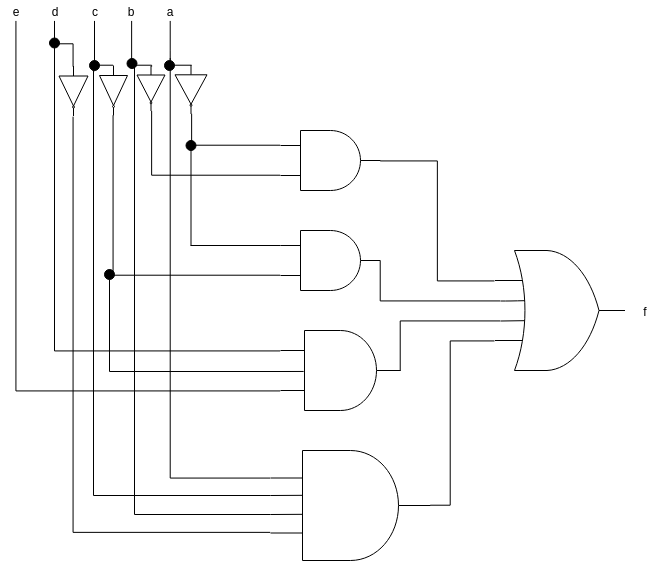
\includegraphics[scale=0.5]{EJ_2/resources/ej_2_minterms_0.png}
    \caption{Circuito l\'ogico seg\'un la expresi\'on m\'inima hallada}
\end{figure}

\begin{figure}[H]
    \centering
    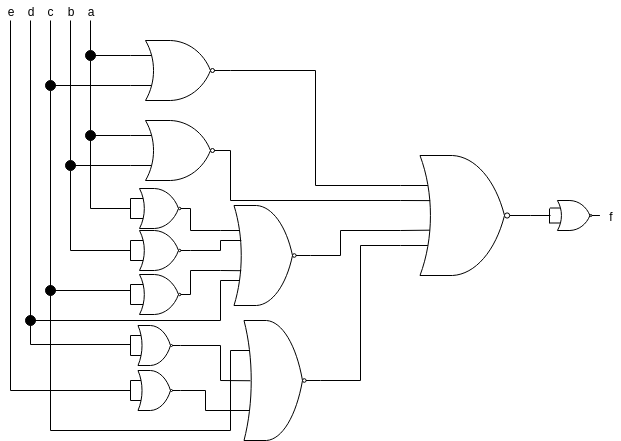
\includegraphics[scale=0.5]{EJ_2/resources/ej_2_minterms_1.png}
    \caption{Circuito l\'ogico implementado s\'olo con compuertas NOR}
\end{figure}

% El desarrollo de la segunda expresión de 4 variables
% usando maxtérminos se realiza en esta subsección
\subsection{Expresi\'on en maxt\'erminos}
En forma an\'aloga con la expresi\'on de los mint\'erminos, se presenta la expresi\'on de maxt\'erminos consignada para ser
desarrollada y simplificada a trav\'es de diferentes m\'etodos. Aqu\'i tambi\'en se emplea el uso de sub\'indices para describir
e identificar los t\'erminos al momento de aplicar las propiedades.

\begin{equation*}
    f(d,c,b,a) = \prod M(0,2,4,7,8,10,12)
\end{equation*}

\subsubsection{Simplificación con Álgebra booleana}

\begin{align*}
f(d,c,b,a) & = \subindex{0} {(d+c+b+a)}
\cdot \subindex{1} {(d+c+\overline{b}+a)}
\cdot \subindex{2} {(d+\overline{c}+b+a)}
\cdot \subindex{3} {(d+\overline{c}+\overline{b}+\overline{a})}
\cdot \subindex{4} {(\overline{d}+c+b+a)} \\
& \cdot \subindex{5} {(\overline{d}+c+\overline{b}+a)}
\cdot \subindex{6} {(\overline{d}+\overline{c}+b+a)}
\end{align*}

Se aplica la propiedad de absorci\'on y, juntando los t\'erminos que son indicados en los sub\'indices de los 
resultantes, luego se llega a la siguiente expresi\'on:

\begin{align*}
f(d,c,b,a) & = \subindex{0,1} {\color{blue} (d+c+a)}
\cdot \subindex{0,2} {\color{brown} (d+b+a)}
\cdot \subindex{0,4} {(c+b+a)}
\cdot \subindex{1,5} {(c+\overline{b}+a)}
\cdot \subindex{2,6} {(\overline{c}+b+a)}
\cdot \subindex{5} {(d+\overline{c}+\overline{b}+\overline{a})} \\
& \cdot \subindex{4,5} {\color{blue} (\overline{d}+c+a)}
\cdot \subindex{4,6} {\color{brown} (\overline{d}+b+a)}
\end{align*}

Nuevamente aplicando absorci\'on con los t\'erminos indicados en los colores azul y marr\'on,
luego queda expresado de la siguiente forma para volver a aplicar la misma propiedad:

\begin{align*}
f(d,c,b,a) & = {\color{blue} (c+a)}
\cdot {\color{brown} (b+a)}
\cdot {\color{blue} (c+b+a)}
\cdot {\color{blue} (c+\overline{b}+a)}
\cdot {\color{brown} (\overline{c}+b+a)}
\cdot {(d+\overline{c}+\overline{b}+\overline{a})} 
\end{align*}

Finalmente absorbiendo estos miembros de las sumas:

\begin{align*}
f(d,c,b,a) & = {(c+a)}
\cdot {(b+a)}
\cdot {(d+\overline{c}+\overline{b}+\overline{a})} 
\end{align*}

\subsubsection{Simplificación con mapas de Karnaugh}

\begin{figure}[H]
    \centering
    \begin{Karnaugh}
    \maxterms{0,2,4,7,8,10,12}
    \minterms{1,3,5,6,9,11,13,14,15}
    \implicantcantons{red}
    \implicant{0}{8}{blue}
    \implicantsol{7}{red}
    \end{Karnaugh}
\end{figure}

De la selecci\'on de los grupos del mapa de Karnaugh se obtiene la siguiente expresi\'on conformada por un producto
de sumas de los maxt\'erminos reducidos por este m\'etodo.

\begin{align*}
f(d,c,b,a) & = {(c+a)}
\cdot {(b+a)}
\cdot {(d+\overline{c}+\overline{b}+\overline{a})} 
\end{align*}

\subsubsection{Expresión desarrollada usando NOR}
En forma an\'aloga a la otra parte del ejercicio la expresi\'on obtenida anteriormente puede ser llevada a una forma donde se haga
uso \'unicamente de operaciones NOR aplicando el teorema de De Morgan.

\begin{align*}
f(d,c,b,a) & = \overline{
    \overline{
        {(c+a)}
        \cdot {(b+a)}
        \cdot {(d+\overline{c}+\overline{b}+\overline{a})} 
    }
}
\end{align*}

\begin{align*}
f(d,c,b,a) & = \overline{
    \overline{(c+a)}
    + \overline{(b+a)}
    + \overline{(d+\overline{c}+\overline{b}+\overline{a})} 
}
\end{align*}

\subsubsection{Circuitos lógicos}

\begin{figure}[H]
    \centering
    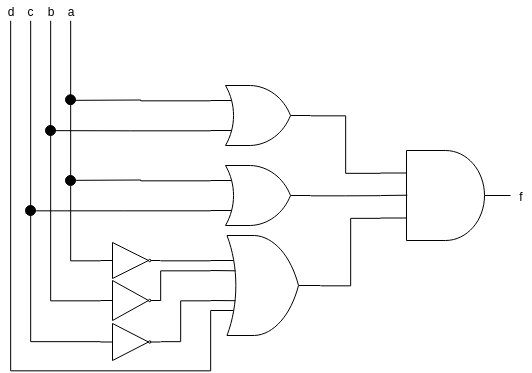
\includegraphics[scale=0.5]{EJ_2/resources/ej_2_maxterms_0.png}
    \caption{Circuito l\'ogico seg\'un la expresi\'on m\'inima hallada}
\end{figure}

\begin{figure}[H]
    \centering
    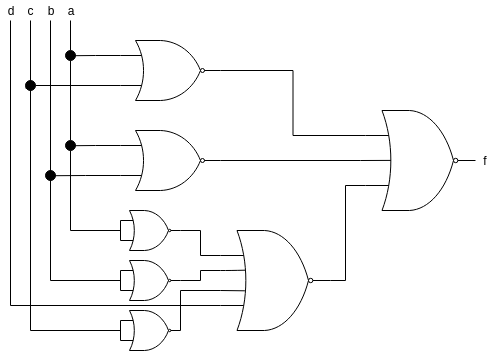
\includegraphics[scale=0.5]{EJ_2/resources/ej_2_maxterms_1.png}
    \caption{Circuito l\'ogico implementado s\'olo con compuertas NOR}
\end{figure}
